% Nama Kelompok : FreeBSD
% Kelas         : D4 Teknik Informatika 1A
% Anggota       :
% 1. Jeremia Wahyudi Sianturi		1174029
% 2. Dwiyulianingsih				1174009
% 3. Arjun Yuda Firwanda			1174008
% 4. Dwi Septiani Tsaniyah			1174003
% 5. Ervanda Rambu Anarky			1174007
% 6. Muh. Rifky	Prananda			1174017
\section{FreeBSD}
	FreeBSD adalah suatu sistem operasi bersifat open source bertipe UNIX bebas yang diturunkan dari UNIX AT\&T lewat cabang Berkeley Software distribution
	BSD. FreeBSD adalah salah satu keluarga BSD yang saat ini banyak digunakan dan dikembangkan pada berbagai kalangan individu,
	perusahaan, dan bahkan universitas. Bila dibandingkan dengan windows FreeBSD relatif lebih sulit dalam penggunaannya, karenya masih bersifat text base
	dalam memberikan command sedangkan windows memiliki GUI yang jauh lebih dibandingkan FreeBSD keunggulan FreeBSD dibanding windows
	adalah kebebasan dalam penggunaannya bahkan pengembangan dari sistem operasi tersebut lisensinya sudah dijamin untuk kebebasan.
	FreeBSD mengoptimalkan penggunaan flatform PC. FreeBSD menyediakan kemudahan dalam penggunaan instalasi dan dukungan yang luas terhadap perangkat keras dalam PC.
	FreeBSD mendukung arsitektur i386 dan Alpha, dan pengembangannya pada beberapa flatform telah dilakukan.
	\ref{index} 
	\begin{figure} [ht]
	\centerline{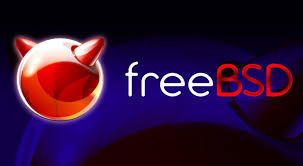
\includegraphics[width=1\textwidth]{figures/index.jpg}}
	\caption{gambarindex}
	\label {index}
	\end {figure}
\subsection{Sejarah}
	menurut \cite{luanmembangun} menyebutkan bahwa :
	Berkeley software distribution diawali dari modifikasi AT\&T Unix software, sebelum berkembang menjadi suatu proyek yang signifikan. Namun sayangnya, AT\&T masih memegang lisensi untuk UNIX dan bertentangan dengan Berkeley Software Design Inc. BSDI yang mengklaim bahwa Berkeley Software Distribution juga termasuk source code AT\&T.
	Kasus lisensi ini sempat dibawa ke pengadilan, dan diproses yang kemudian  menghasilkan bahwa Bill Jolitz berwenang untuk mengambil bagian dari software yang bukan berasal dari AT\&T dan kemudian mengembalikannya menjadi free UNIX. Ini merupakan sebuah awal baru dari lahirnya modern BSD.
	Dalam pengembangannya FreeBSD melibatkan begitu banyak pihak yang notabene merupakan programmer individu berkemampuan tinggi yang dikenal sebagai commiters. Commiters ini dipilih oleh FreeBSD core team dan memiliki wewenang langsung untuk melakukan suatu perubahan-perubahan pada system yang  berjalan.
	FreeBSD lahir pada tahun 1992 saat Jordan K. Hubbard, Rob Grimes, dan Nate Williams merilis sebuah paket yang dikenal dengan unofficial 386BSD patchkit. Dari sana lahirlah suatu mekanisme yang membentuk 386BSD 0.5 1/2, akan tetapi pada 1993 Jolitz mencabut persetujuan pada proyek tersebut dan melahirkan FreeBSD. 
	Jordan K Hubbard dan David Greenman kemudian membentuk suatu kerjasama untuk mempersiapkan sebuah proyek CDROM FreeBSD versi 1.0 berbasis Net/2 yang telah dirilis pada bulan desember tahun 1993, setelah itu pada bulan November 1994 versi kedua dari FreeBSD dirilis yaitu versi 2.0 yag tidak lagi 
	berbasis Net/2 tetapi telah diupgrade menjadi berbasis 4.4BSD BSD dibuat, dikembangkan serta digunakan secara bebas sebagai perlawanan terhadap lisensi UNIX yang dimiliki oleh AT\&T. oleh karena itu BSD mempunyai lisensi sendiri yang memungkinkan setiap individu bebas melakukan pengembangan dan
	FreeBSD telah digunakan diseluruh penjuru internet oleh beberapa perusahaan yang memiliki orientasi pada internet. sebagai contohnya saat ini the \"babybell\" US west menggunakan FreeBSD untuk menjalankan operasional internet. IBM, Nokia, dan banyak perusahaan hardware menggunakan FreeBSD pada embedded system.
	dalam kenyataannya jika sebuah perusahaan serius untuk melakukan manajemen bandwich internet, kemungkinan besar sistemnya menjalankan FreeBSD.
	saat ini FreeBSD memiliki hampir 300 developer. comitters mempunyai hak read-and-write atas master source code dan dapat men-develop, debug, atau memperbaiki kulaitas bagian yang dianggap penting.
	sebagai contoh, developmen networking dibahas dalam milis-milis yang banyak tersebar di media sosial ada pula beberapa chanel IRC untuk mendiskusikan banyak hal mengenai FreeBSD.
	para committers bertanggung jawab agar FreeBSD tetap berjalan dan memabah fitur baru serta mengevaluasi patch yang dikirim oleh para kontributor. 
	hingga akhirnya FreeBSD memiliki users yang jauh lebih banyak karena kita dapat mendownload keseluruhan FreeBSD dengan gratis dan tidak perlu register, upgrade atau mengirim email ke mailing list.

\subsection{VarianFreeBSD}
	Varian dari FreeBSD kami mendapatkan referensi dari \cite{nugroho2015analisis} yang kami kembangkan menjadi :
	FreeBSD memiliki dua versi saat dirilis. versi tersebut antara lain versi-CURRENT dan versi-STABLE. selain itu varian FreeBSD juga ada UNIX FreeBSD, NETBSD, OpenBSD, UNIX lainnya, dan AIX yang dikenal dapat dijalankan pada banyak jenis arsitektur, dan FreeBSD yang mendukung flatform X86, AMD64, IA64, SPARC64, dan Alpha.
	FreeBSD 6.0 dikenal dengan stabilitas, performa, dan keamannanya sehingga digunakan oleh banyak perusahaan di seluruh dunia. rilis UNIX freeBSD yang digunakan saat ini adalah versi 6.2. 
	Sebenarnya masih banyak lagi jenis-jenis sistem operasi yang dapat dikatakan berbasis dengan FreeBSD seperti IRIX, HPUX, LINUX, Sun Solaris, Mac OS X, BSD/OS dan juga masih ada lagi yang belum disebutkan tapi mungkin karena berikut merupakan kesimpulan sederhana jadi tidak dijelaskan secara semua atau dapat dikatakan menyeluruh. 
	Jadi dapat ditarik bahwa banyak jenis-jenis dari OS FreeBSD yang telah disebutkan.
	pengembangan gentoo/FreeBSD menggunakan versi ini, sedangkan  pengembangan dengan versi lama telah dihentikan dan tidak lagi didukung. pada varian BSD NETBSD dan OPENBSD memiliki modal pengembangan sistem operasi yang terbuka akan tetapi memiliki susanan tertentu yaitu :
	1. contributor, adalah developer yang menulis kode, patch atau dokumentasi, akan tetapi tidak memiliki hak untuk menulis atau membuat suatu file dalam source tree. jika pekerjaan yang mereka lakukan ingin dimasukkan maka harus diperiksa terlebih dahulu oleh committers atau dengan persetujuan beberapa orang committers
	2. commiters adalah developer yang memiliki hak menulis dan mengakses source tree, dalam lingkup cvs, memiliki hak commit secara tipikal dan hanya bekerja dalam bagian terpilih di suatu proyek.
	3. coreteam memiliki wewenang untuk membimbing secara keseluruhan arah dan tujuan proyek, dan membuat keputusan akhir dalam kasus berselisih paham antar developer mengenai source code atau hal-hal lain. OpenBSD tidak memiliki coreteam secara formal namun Theo De Raadt bertugas sebagai pemimpin proyek.
	setap orang dapat menjadi contributor dengan mengirimkan patch atau membenarkan kesalahan penulisan dalam sebuah halaman manual orang yang mengkontribusikan banyak hal, atau berkompeten dalam suatu proyek akan dipeomosikan menjadi commiters yang ditujukan untuk menjaga committers yang lain memeriksa terlalu banyak hal dalam waktu yang sama.
\subsubsection{versi-CURRENT}
	versi-CURRENT merupakan versi yang pertama kali dirilis biasanya versi ini dipakai oleh para develover yang sudah mahir mengenai
	cara kerja dari FreeBSD agar dapat menemukan berbagai bugs paska produksi. setelah versi-CURRENT diperbaiki maka versi tersebut
	akan menjadi versi stable yang siap digunakan karena dalam versi-CURRENT kurang familiar bagi pengguna baru FreeBSD.
	\ref{freebsd} 
	\begin{figure} [ht]
	\centerline{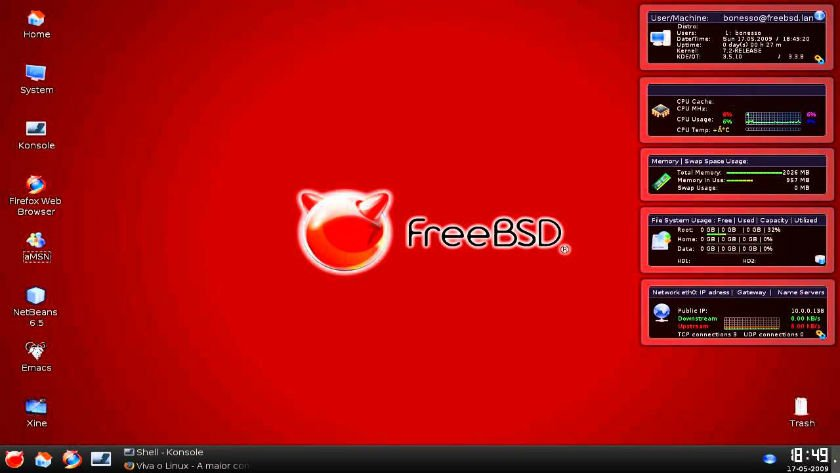
\includegraphics[width=1\textwidth]{figures/freebsd.jpg}}
	\caption{gambarindex}
	\label {freebsd}
	\end {figure}
\subsection{Sejarah}
\subsubsection{versi-STABLE}
	versi-STABLE adalah versi pengembangan ddari versi sebelumnya yaitu versi-CURRENT yang dianggap kurang familiar.
	versi-STABLE siap digunakan oleh siapapun yang baru mencoba FreeBSD karena versi sebelumnya hanya ditujukan kepada
	orang yang mahir dalam mengidentivikasi masalaah yang muncul pada versi tersebut.
\subsubsection{NETBSD}
	NetBSD dapat juga dikatakan mirip dengan FreeBSD dalam berbagai macam bentuk dan aspek. Kedua proyek ini saling berbagi source code dan developer. 
	Tujuan paling utama dari NetBSD adalah membuat sistem operasi yang dapat diporting ke berbagai macam plattform hardware. 
	Sebagai contohnya bahwa NetBSD dapat berjalan di berbagai macam plattform hardware yaitu : bahwa NetBSD dapat berjalan di VAXes, PocketPC, Alpha server, dan Compaq iPaq. Bahkan NetBSD dapat berjalan juga pada hardware yang belum ada (belum diluncurkan). 
	Source code NetBSD diberikan secara bebas, sama seperti pendahulunya, FreeBSD.
\subsubsection{openBSD}
	OpenBSD merupakan cabang dari NetBSD mulai tahun  1996, tujuan utam dari OpenBSD adalah membuat OS BSD yang aman. 
	OpenBSD adalah BSD yang pertama kali men-suport hardware-accelerated crytography {membolehkan untuk men-encrypt dan decrypt informasi pada waktu yang singkat, para developenya sangat bangga karena faktanya, default instalasi OpenBSD tidak dapat di-hack selama kira-kira 4 tahun.
\subsubsection{UNIXFreeBSD}
	FreeBSD dapat dikatakan mirip dengan sistem operasi Unix yang bebas {berlisensi}. Pada tahun 1993 ketika pengembangan 386BSD dihentikan, maka lahirlah dua proyek baru yang satu dikenal dengan nama Net BSD, yang dikenal dapat dijalankan pada banyak jenis arsitektur, 
	dan yang satunya lagi dikenal dengan sebutan FreeBSD yang mendukung platform x86, amd64, ia64, sparc64 dan alpha. 
	Free BSD 6.0 dikenal juga denagn stabilitas, performa dan keamanannya sehingga sering digunakan oleh perusahaan-perusahaan terkenal yang ada di seluruh dunia. 
	Saat ini unix FreeBSD yang digunakan adalah versi 6.2. Dan sebentar lagi juga akan keluar pengembangan  Gentoo/FreeBSD versi terbaru, sedangkan versi lama yang ingin dikembangkan malah diberhentikan proyeknya dan tidak didukung sama sekali pembentukannya. 
	Pasti kita semua bertanya-tanya apa itu Gentoo/FreeBSD? Baiklah akan dijelaskan bahwa Gentoo/FreeBSD adalah subproyek dari proyek Gentoo/Alt, Yang tujuannya hanya untuk menyediakan sistem operasi FreeBSD berkemampuan penuh dengan mengambil rancangan dari Gentoo Linux, seperti sistem unit dan sistem manajemen paket Portage.
\subsubsection{UNIXLainnya}
	Masih ada beberapa UNIX OS di luar sana, beberapa bahkan menyewa nama trademark dari UNIX sehingga mereka dapat menyebut diri mereka itu UNIX
\subsubsection{AIX}
	Salah satu pesaing ketat dari UNIX adalah IBM AIX. AIX mengklaim bahwa mereka mempunyai journaling filesystem terbaik seperti, mampu mencatat seluruh disk transaction yang terjadi, sehingga mereka mampu me-recover system tanpa banyak masalah kemampuan ini meningkatkan reliability. 
	Dan AIX juga berbasis BSD.
\subsection{Tujuan}
	Tujuan dari adanya software ini adalah untuk menyediakan software yang tentu saja dapat digunakan dalam berbagai kepentingan dengan mudah dan gratis (free). karena software ini disediakan dengan gratis dan dapat digunakan oleh siapa saja termasuk untuk meraih kepentingan komersil, 
	source kode yang tersedia dengan gratis siapun dapat meningkatkan  peforma melalui free bsd ini atau memungkinkan bug mensubmit source codenya dan dapat digunakan sesuai dengan keinginan si pengguna.
	Tujuan dari adanya versi-CURRENT dan versi-STABLE adalah untuk memberitahukan fixed bugs bagi para pengguna
	dan meyakinkan pengguna dengan fitur - fitur terbaru dan masalah yang telah diatasi. selain perbedaan diantara versi-CURRENT dan versi-STABLE
	pemberian nama dari versi-STABLE juga telah dibuat sedemikian rupa hingga para penggguna tahu  perbaikan - perbaikan yang telah dilakukan.
\subsection{kegunaanFreeBSD}
	pada saat ini FreeBSD dikenal sebagai network administrator operating system karena FreeBSDberjalan dengan cepat dan telah banyak tersedia berbagai networking tools. selain itu, FreeBSDdapat berjalan denngan cepat dan efisien didalam sebuah laptop untuk menjalankan aplikasi perkantoran, atau sebagai email client maupun email database.
	instalasi dari FreeBSD dapat dikatakan cukup mudah bagi yang sudah pernah menginstall system operasi windows.
\subsection{keuntungandankelemahan}
	keuntungan dan kelemahan kami mengambil referensi dari : \cite{nugroho2015analisis}
	keuntungan :
	1. FreeBSDdapat berjalan lebih cepat daripada LINUX dalam beberapa bagian misalnya sebagai server NFS
	2. dalam aplikasi server secara prinsip BSD sama baiknya dengan LINUX
	kelemahan :
	1. FreeBSD tidak dapat digunakan pada microkanal lama
	2. FreeBSD tidak dapat mendukung ISA-plug-and-play-card
	3. FreeBSD tidak bisa menandingi perkembangan LINUX yang cepat karena kurangnya developer
	4. FreeBSD belum jelas masa depannya untuk server database
\subsection{Kesimpulan}
	Dari penjelasan diatas dapat disimpulkan bahwa FREEBSD mempunyai banyak fitur-fituryang dapat dipelajari satu per satu. Dan ada kelebihan, kekurangan yang ada di FREEBSD, diataranya banyaknya tersedia aplikasi dan program file gratis. 
	Mudah di kustomisasi atau dapat dirubah-rubah secara bebas. Freebsd mempunyai fitur multiuser, bersifat opensource, memiliki sistem software third-party yang memberikan kemudahan yang berarti bagi para user untuk menambah atau menghapus aplikasi-aplikasi.
	Para user cukup mengeksekusi satu baris perintah dan aplikasi-aplikasi dengan sendirinya di download dan diinstal secara otomatis, sehingga tugas-tugas didalam system Freebsd menjadi mudah dan praktis. 
	Dari beberapa kelebihan diatas secara progaming Freebsd dapat dikatakan system yang dapat mempermudah user dalam menggunakan dalam berbagai tugas-tugas system operasi.
	Di dalam Freebsd terdapat kekurangan juga, diantaranya relatif penggunaannya sulit karena masih dalam bentuk text base dalam mengcommandnya, artinya dalam memerintahnya masih sulit. Tidak mendukung ISA plug and play chard, artinya tidak dapat memasang dan memainkan. 
	Kecilnya basis developer dan pemakai yang mencari bug/kelemahan program.
	Operating sistem ini dinamakan freeBSD karena software ini gratis untuk digunakan oleh siapapun termasuk untuk kepentingan komersial, source code yang tersedia dengan gratis, siapapun dapat meningkatkan performa freeBSD ini atau menemukan bug
	(Pengertian bug adalah kesalahan pada komputer baik disebabkan oleh perangkat lunak ataupun perangkat keras sehingga komputer tidak bekerja dengan semestinya ) untuk mensubmit souce codenya, kata ‘free’ dapat diartikan sebagai gratis, atau dapat digunakan sesuai keinginan user.
	FreeBSD dikenal sebagai network administrator operating system karena FreeBSD berjalan dengan cepat dan telah banyak tersedia berbagai networking tools. 
	selain itu, FreeBSD dapat berjalan denngan cepat dan efisien didalam sebuah laptop untuk menjalankan aplikasi perkantoran, atau sebagai email client maupun email database.
	FreeBSD dapat dikatakan cukup mudah bagi yang sudah pernah menginstall system operasi windows.
	FreeBSD dapat berjalan di personal komputer yang menggunakan sistem arsitektur Intel. Artinya dapat mendapatkan secara gratis tanpa berbayar.
